\author{Ethan Grant uni: erg2145}
\title{P-Set 1 Adv Econometrics}
\date{\today}

\documentclass{article}
\usepackage{amsmath}
\usepackage{graphicx}
\begin{document}
	\maketitle
	\begin{enumerate}
		\item
			\begin{enumerate}
				\item
				\newpage
				
				average value for each vector comes out to:\newline E =  0.014003698, \t  0.054311176, \t 0.004744255, \t -0.046776593,\t  0.044269689
				\newline
				This is in line with what i predicted as all the values are close to zero.
				\newline \newline
				Var(X) =
				\newline           [,1]      [,2]     [,3]     [,4]     [,5]\newline
				[1,] 0.9177694 0.9598261 1.017785 1.017376 1.017693\newline
				[2,] 0.9598261 1.9786326 2.010952 2.035977 2.079679\newline
				[3,] 1.0177846 2.0109515 2.989345 3.007466 3.063471\newline
				[4,] 1.0173761 2.0359771 3.007466 4.045282 4.071903\newline
				[5,] 1.0176934 2.0796790 3.063471 4.071903 5.147865\newline
				\newline
				this is also what I predicted as variance covariance matrix increases as you move toward bottom element
				\newline
				\item
				see code for implementation
				\item
				Var(reg\$betas\_n\_1000) \newline
				              [,1]          [,2]          [,3]          [,4]          [,5]\newline
				              [1,]  4.492060e-03 -2.109167e-03 -3.271328e-04  9.6336e-05  2.7132e-05\newline
				              [2,] -2.109167e-03  4.305546e-03 -2.177376e-03  3.7844e-05 -4.2901e-05\newline
				              [3,] -3.271328e-04 -2.177376e-03  4.299288e-03 -1.9269e-03 -4.9570e-05\newline
				              [4,]  9.633620e-05  3.784497e-05 -1.926927e-03  3.8629e-03 -1.9412e-03\newline
				              [5,]  2.713261e-05 -4.290154e-05 -4.957046e-05 -1.9412e-03  1.9570e-03\newline
				              \newline
				$\sigma^{2}$=2 as defined by creation of variables \newline
				
				thus $2*(X'X)^{-1}$= \newline
				[,1]          [,2]          [,3]          [,4]          [,5]\newline
				[1,]  4.451362e-03 -1.955891e-03 -2.560439e-04 -4.1618e-05  9.5782e-05\newline
				[2,] -1.955891e-03  4.0460e-03 -1.9976e-03  1.866394e-05 -7.537309e-05\newline
				[3,] -2.560439e-04 -1.997684e-03  4.0690e-03 -1.8713e-03 -8.352393e-05\newline
				[4,] -4.161810e-05  1.866394e-05 -1.8713e-03  3.7301e-03 -1.833926e-03\newline
				[5,]  9.578261e-05 -7.537309e-05 -8.352393e-05 -1.8339e-03  1.8992e-03\newline
				\newline
				These values are very similar as is expected
				\item
				N=10 \newline
				mean($\hat{\sigma}_{1,b}^{2}$)= 0.9895263   \newline
				mean($\hat{\sigma}_{2,b}^{2}$)= 1.979053   \newline
				N=20 \newline
				mean($\hat{\sigma}_{1,b}^{2}$)= 1.4700532   \newline
				mean($\hat{\sigma}_{2,b}^{2}$)= 1.960071   \newline
				N=100 \newline
				mean($\hat{\sigma}_{1,b}^{2}$)= 1.8840889   \newline
				mean($\hat{\sigma}_{2,b}^{2}$)= 1.983251   \newline
				N=1000 \newline
				mean($\hat{\sigma}_{1,b}^{2}$)= 1.9884902    \newline
				mean($\hat{\sigma}_{2,b}^{2}$)= 1.998483   \newline
				\newline
				Both formulas eventually converge upon the true average (2), but the adjusted sigma that accounts for bias ($\hat{\sigma}_{2,b}^{2}$) gets close to the true value even when n=10 while the other is very far away at that point
				\item
				\begin{center}
					n=10 \newline
					 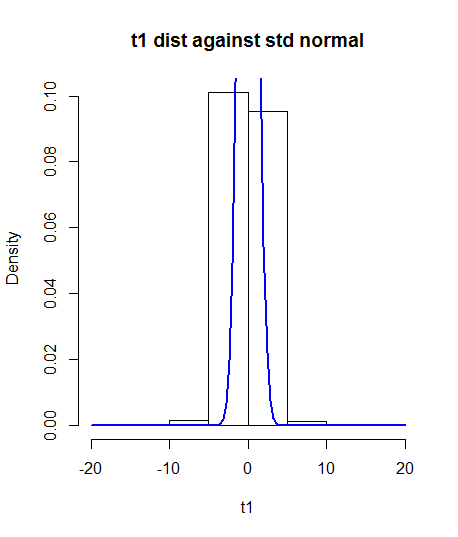
\includegraphics[scale=.5]{t1_10}
						 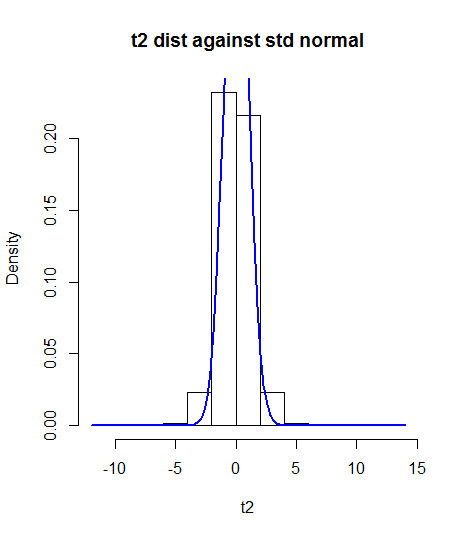
\includegraphics[scale=.5]{t2_10}
							\newline
							n=20 \newline
							 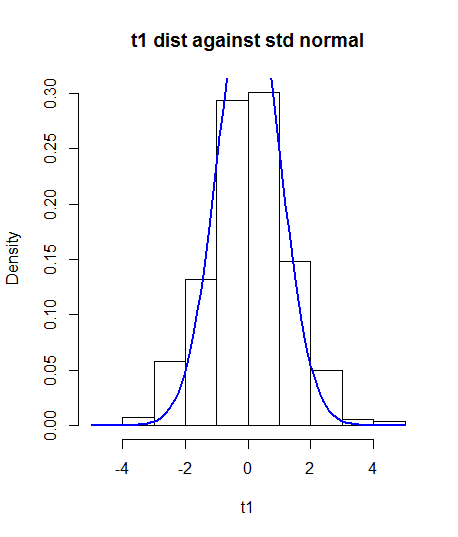
\includegraphics[scale=.5]{t1_20}
								 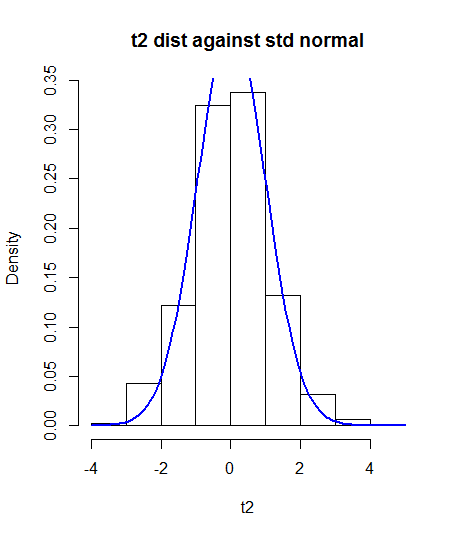
\includegraphics[scale=.5]{t2_20}
									\newline
									n=100 \newline
									 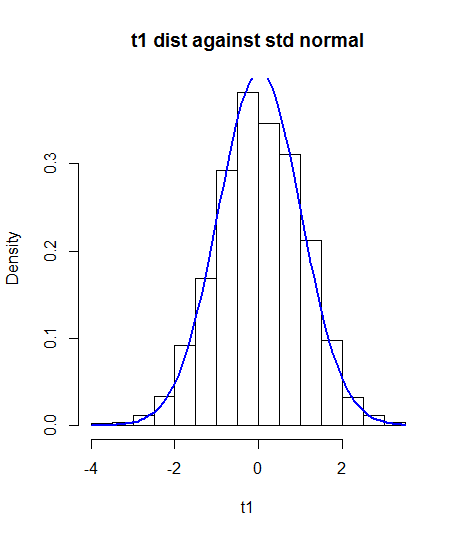
\includegraphics[scale=.5]{t1_100}
										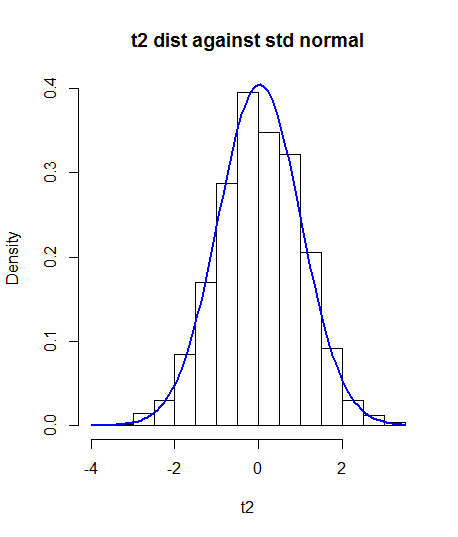
\includegraphics[scale=.5]{t2_100}
										\newline
										n=1000 \newline
										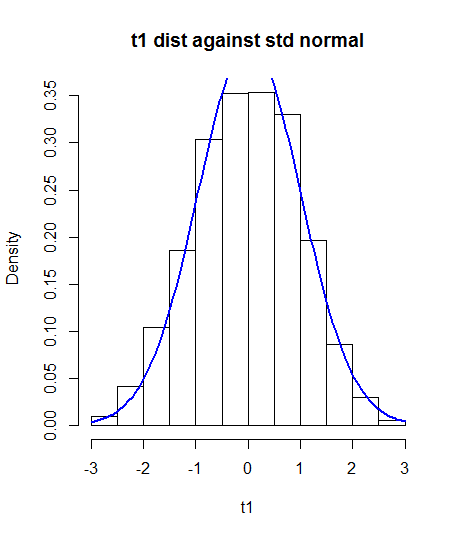
\includegraphics[scale=.5]{t1_1000}
										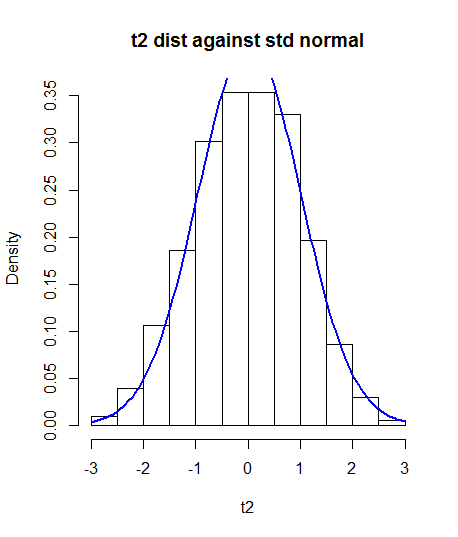
\includegraphics[scale=.5]{t2_1000}
				\end{center}
				
				
				N=10 reject .389\newline
				N=20 reject .582\newline
				N=100 reject .997\newline
				N=1000 reject 1\newline
				\newline
				As N increases the test rejects more and more which is what you would want as the null hypothesis that $\beta_{0}=0$ is false. I conclude that the test is consistent
			\end{enumerate}
	\item
			\begin{enumerate}
				\item see code
				\item beta\_hat = [3.98,.134,.00029] \newline
				mean(residual) = 5.127 e-15 \newline
				var(residual) = .297 \newline
				mean(residual\_from\_maker) = 3.68 e -15 \newline
				sd(residual\_from\_maker) = .544 \newline
				\begin{center}
					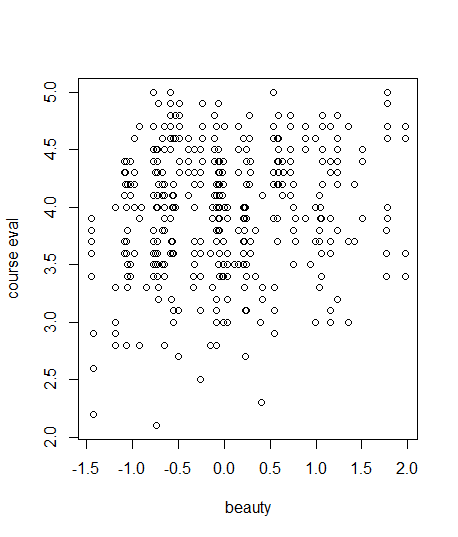
\includegraphics{scatterplot}
				\end{center}
				 
				\item 
				FW estimates = [.134,.00029] \newline
				
				The OLS estimates (reported in part ii) are the same as the FW estimates though the FW estimates do not include the intercept part of the vector.
				\item 
				variance covariance matrix:
				\newline
				              intercept        beauty           age\newline
				              intercept  0.0178836140 -1.319840e-03 -3.564487e-04\newline
				              beauty    -0.0013198398  1.138662e-03  2.728914e-05\newline
				              age       -0.0003564487  2.728914e-05  7.369971e-06\newline
	            \newline
	            CI beta1 = [.0679,.2002] \newline
	            CI beta2 = [-.005,.0056] \newline
	            \newline
	            These seem like reasonable confidence intervals and both are reasonably tight around the original value meaning the estimates are decently close to the true value
				\item
				uncentered\_r\_squared = .981   \newline
				centered\_r\_squared = .0357  \newline
				\newline
				The uncentered r squared is very close to 1 suggesting that the regression we have is a very good fit, while the centered r squared is very close to 0 suggesting we have a bad fit. This difference makes it important which one we prefer \newline
				\newline
				I prefer the centered R squared because it is based on the assumption that there is some intercept not equal to zero which looking at the data seems very reasonable. Additionally looking at the scatterplot it does not seem like the variation is explained very heavily by the regressors indicating that such a high r squared is not accurate
				
				\item
				mean(residuals) = 3.68 e-15 \newline
				cor(residual, X[,'beauty']) = -2.92 e-15 \newline
				cor(residual, X[, 'age']) = -6.42 e-15 \newline
				\newline
				These do make sense given what we have seen in class b/c our assumption is that E[u|x] = 0 which means that the mean of the residuals should be zero which we are very close to achieving here. Additionally the correlation being very close to zero also makes sense because if there was a correlation that implies that there is more information about that error (and thus y) that is contained in either of the X values that is not currently being used. This goes against our assumptions and the math so we want these values to be very very close to zero which they are.
			\end{enumerate}	
		
	\end{enumerate}
\end{document}		
		